\documentclass[../thesis/thesis.tex]{subfiles}
\renewcommand{\baselinestretch}{1.5}\selectfont
\graphicspath{{../figs/ch5-nlbmunc/}}

\begin{document}
	
\onlyinsubfile{\setcounter{chapter}{4}}

\begin{refsection}
\chapter[Prop. Meas. Unc. To Nonlinear Behavioural Models]{Propagating Measurement Uncertainty into Nonlinear Behavioural Models}
\section{Introduction}

A brief coverage of the requirement for behavioural models and the history. Talk about the benefits of adding confidence information to simulations during amplifier design.

yield analysis in circuit simulation
characterisation of amplifiers for digital pre-distortion \cite{Verspecht_2013,Kaur_2012}



\section{Nonlinear Behavioural Models}
\subsection{The Volterra Model}
\subsection{X-Parameters}
\subsection{The Cardiff Model}
\subsection{X-Parameter Extraction Procedure}
\section{Design and Simulation using Nonlinear Behavioural Models Incorporating Measurement Uncertainty}

The NIST MUF was used to perform the calibration of electromagnetic wave parameters measured using a Keysight Technologies 67 GHz N5247A PNA-X LSNA. The DUT was an internally matched Analog Devices HMC342LC4 low noise amplifier \cite{hittite_amp} mounted on a connectorised evaluation board. This amplifier has a typical gain of 19 dB and a \mbox{1-dB} compression point at approximately 9 dBm output power at 25 GHz. To obtain results showing both the linear and nonlinear regimes of operation, the source power was swept between -22 dBm and -2 dBm in 0.25 dB steps. The fundamental frequency was set at 25 GHz, with a harmonic at 50 GHz also measured. The evaluation board used 2.92 mm precision connectors, connected via adapters to cables with 2.4 mm precision connectors. The calibration plane was located between the cables and the adapters (i.e. the adapters were included as part of the DUT), and the measurement setup had a nominal impedance of 50-$\Omega$. The intermediate frequency bandwidth (IFBW) was set to 10 Hz. The built-in X-parameter measurement routine was used and configured to extract cross-frequency terms between both harmonics using measurements at 4 extraction tone phases (this is the default setting). A photograph of the setup is shown in \figurename{ \ref{ch5_fig_setup}}.

\begin{figure}[t]
	\centering
	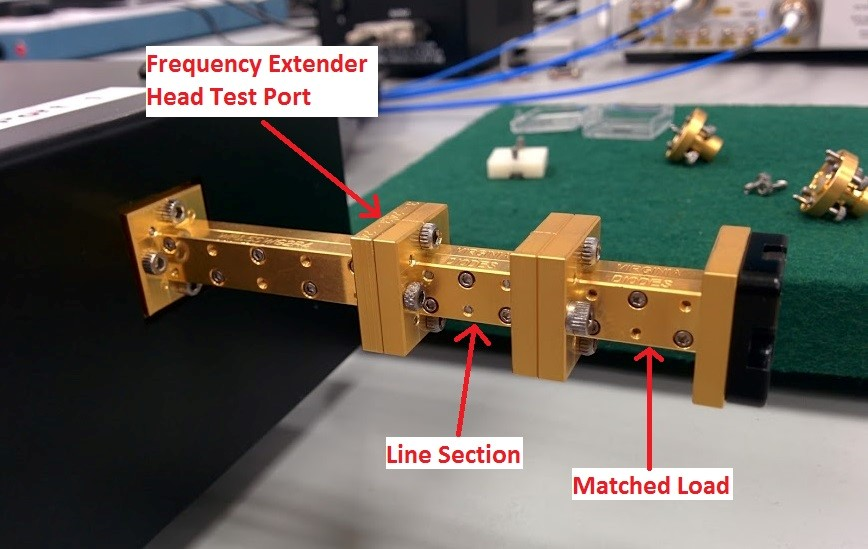
\includegraphics[width=\linewidth]{setup}
	\caption{The measurement setup used for extracting X-parameters from the DUT. Shown is the PNA-X LSNA (A), the phase reference comb generator (B), the phase calibration comb generator (C), the power meter (D), and the connected DUT (E).}
	\label{ch5_fig_setup}
\end{figure}

Uncertainties are propagated through all steps of the calibration by the MUF. We have included uncertainties present in the definitions and measurements of the passive calibration standards, the power meter calibration and measurement, the phase reference characterization and measurement, cable flexure, and connection repeatability of all calibration steps. Uncertainty due to random noise in the high-dynamic range receivers was omitted as it has been shown to be negligible with respect to that arising from other error sources in LSNA measurements \cite{Blockley_2007}.

The MUF supports several calibration algorithms, and for this measurement the multiline TRL calibration algorithm \cite{Engen_1979, Marks_1991} was chosen to allow direct dimensional traceability to national measurement standards. The calibration standards used were from a 1.85 mm precision coaxial calibration kit (Rosenberger RPC-1.85 LRL). Table \ref{ch5_table_passivestds} gives the dimensions of the line standards used for the calibration. To include the effect of connector repeatability on the passive calibration, each standard was measured several times with the connector oriented differently. These measurements were passed to a MUF program (``Combine'') which produces a mean value with an associated uncertainty.

\begin{table}[]
	\centering
	\caption{Nominal values and standard uncertainties for the TRL coaxial line standards.}
	\label{ch5_table_passivestds}
	\begin{tabular}{ccc}
		\hline
		Dimension         & Line 1 value (mm) & Line 2 value (mm) \\ \hline
		Line length       & 13.004 $\pm$ 0.003 & 14.913 $\pm$ 0.003 \\
		Line inside dia.  & 0.803 $\pm$ 0.001 & 0.803 $\pm$ 0.008 \\
		Line outside dia. & 1.850 $\pm$ 0.005 & 1.850 $\pm$ 0.005 \\ \hline            
	\end{tabular}
\end{table}

The power meter measurement, as part of the absolute calibration, measures the amplitude of the waves. The calibration model for the power meter itself is defined in \cite{Keysight_2017} and includes the reference oscillator mismatch, the reference oscillator power uncertainty, the zero-set error, the zero carry-over error, the instrumentation error, and error in the power sensor calibration factor. The estimates and uncertainties used for these parameters in the calibration are shown in Table \ref{ch5_table_powerunc} and are derived from specifications supplied by the manufacturer. The mismatch of the power sensor was also measured using a calibrated VNA and included in the absolute calibration. Connector repeatability was assessed for this measurement in the same way as for the passive standards.

\begin{table}[]
	\centering
	\caption{Standard uncertainties for power meter uncertainty contributions derived in \cite{Keysight_2017}}
	\label{ch5_table_powerunc}
	\begin{tabular}{cc}
		\hline
		Contribution                           & Standard uncertainty \\ \hline
		Reference oscillator mismatch          & 0.2\%                \\
		Reference oscillator power uncertainty & 0.6\%                \\
		Zero-set error                         & 0.5\% meter full scale \\
		Zero carry-over error                  & 0.2\% meter full scale \\
		Instrumentation error                  & 0.5\% meter full scale \\
		Calibration factor error               & 0.024               \\ \hline
	\end{tabular}
\end{table}

In order to complete the absolute calibration, the phase must also be calibrated. This is performed using a harmonic phase reference, which for this calibration was provided by a Keysight Technologies 67 GHz comb generator\cite{Keysight_2014}. This device supplies a stable and repeatable train of pulses, which creates a frequency comb (aligned to the calibration frequencies) to be measured by the LSNA. The phase uncertainties are given in Table \ref{ch5_table_phaseunc} and were obtained through characterization with a sampling oscilloscope at NIST, which is traceable to national measurement standards via electro-optic calibration \cite{Reader_2008, Hale_2009}.

\begin{table}[]
	\centering
	\caption{Nominal phase and standard uncertainty for harmonic phase reference at calibration frequencies}
	\label{ch5_table_phaseunc}
	\begin{tabular}{ccc}
		\hline
		Frequency (GHz) & Characterized phase (deg.) & Measured phase (deg.)\\ \hline
		25 & 181.5 $\pm$ 0.4 & -16.8 $\pm$ 1.5 \\ 
		50 & 170.8 $\pm$ 1.0 & 61.0 $\pm$ 2.5 \\ 
		\hline
	\end{tabular}
\end{table}

\subsection{X-Parameter Uncertainties}

In this example we used Monte Carlo with 1000 samples to propagate uncertainty to the X-parameters of the DUT. This required 8 hours of processing for the calibration and a further 8 hours of processing for the X-parameter extraction.
A histogram is provided in \figurename{ \ref{ch5_fig_hist}} showing good agreement between the Monte Carlo and sensitivity analysis. This level of agreement is typical for all of the extracted X-parameters.

The estimated values and standard uncertainties from the Monte Carlo analysis for the magnitude and phase of a sample of X-parameter terms are shown in \figurename{ \ref{ch5_fig_summaryplots}}. It can be seen in all plots that there is a clear change in uncertainty for several X-parameters as the DUT transitions between the linear and nonlinear regimes.

The phase noise seen at lower powers in the estimate of $X^\textrm{T}_{2,1;2,2}$ is not accompanied by an increase in measurement uncertainty. This suggests that it arises from the extraction routine, which contributes another source of uncertainty not studied in this paper. By design, the $X^\textrm{T}$ parameters are negligible in the linear regime, and so this effect will have little contribution when the model is used.

\begin{figure}
	\centering
	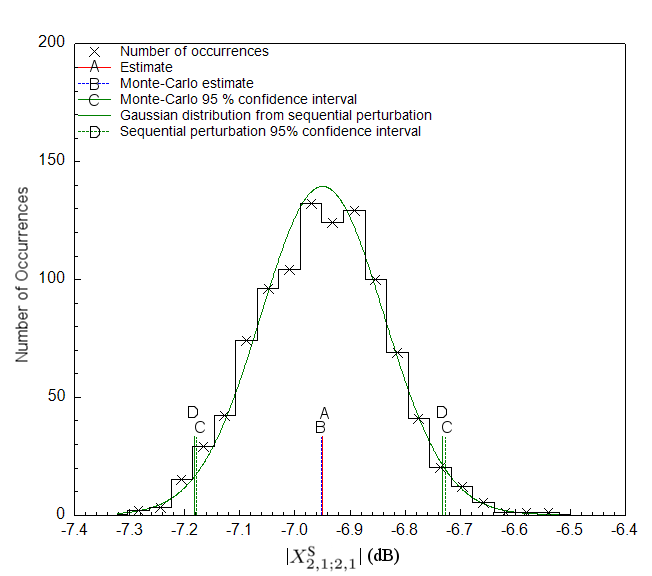
\includegraphics[width=0.8\textwidth]{hist}
	\caption{Histogram comparing the Monte Carlo and sequential perturbation uncertainty results for $X^\textrm{S}_{2,1;2,1}$ (25 GHz) of the DUT at -2.4 dBm source power. The vertical line in the center of the plot (A) shows the nominal value (estimate), (B) shows the Monte Carlo average, and (C, D) show the Monte Carlo and sequential perturbation 95\% confidence intervals, respectively.}
	\label{ch5_fig_hist}
\end{figure}

\begin{figure}
	\centering
	\begin{subfigure}{0.45\textwidth}
		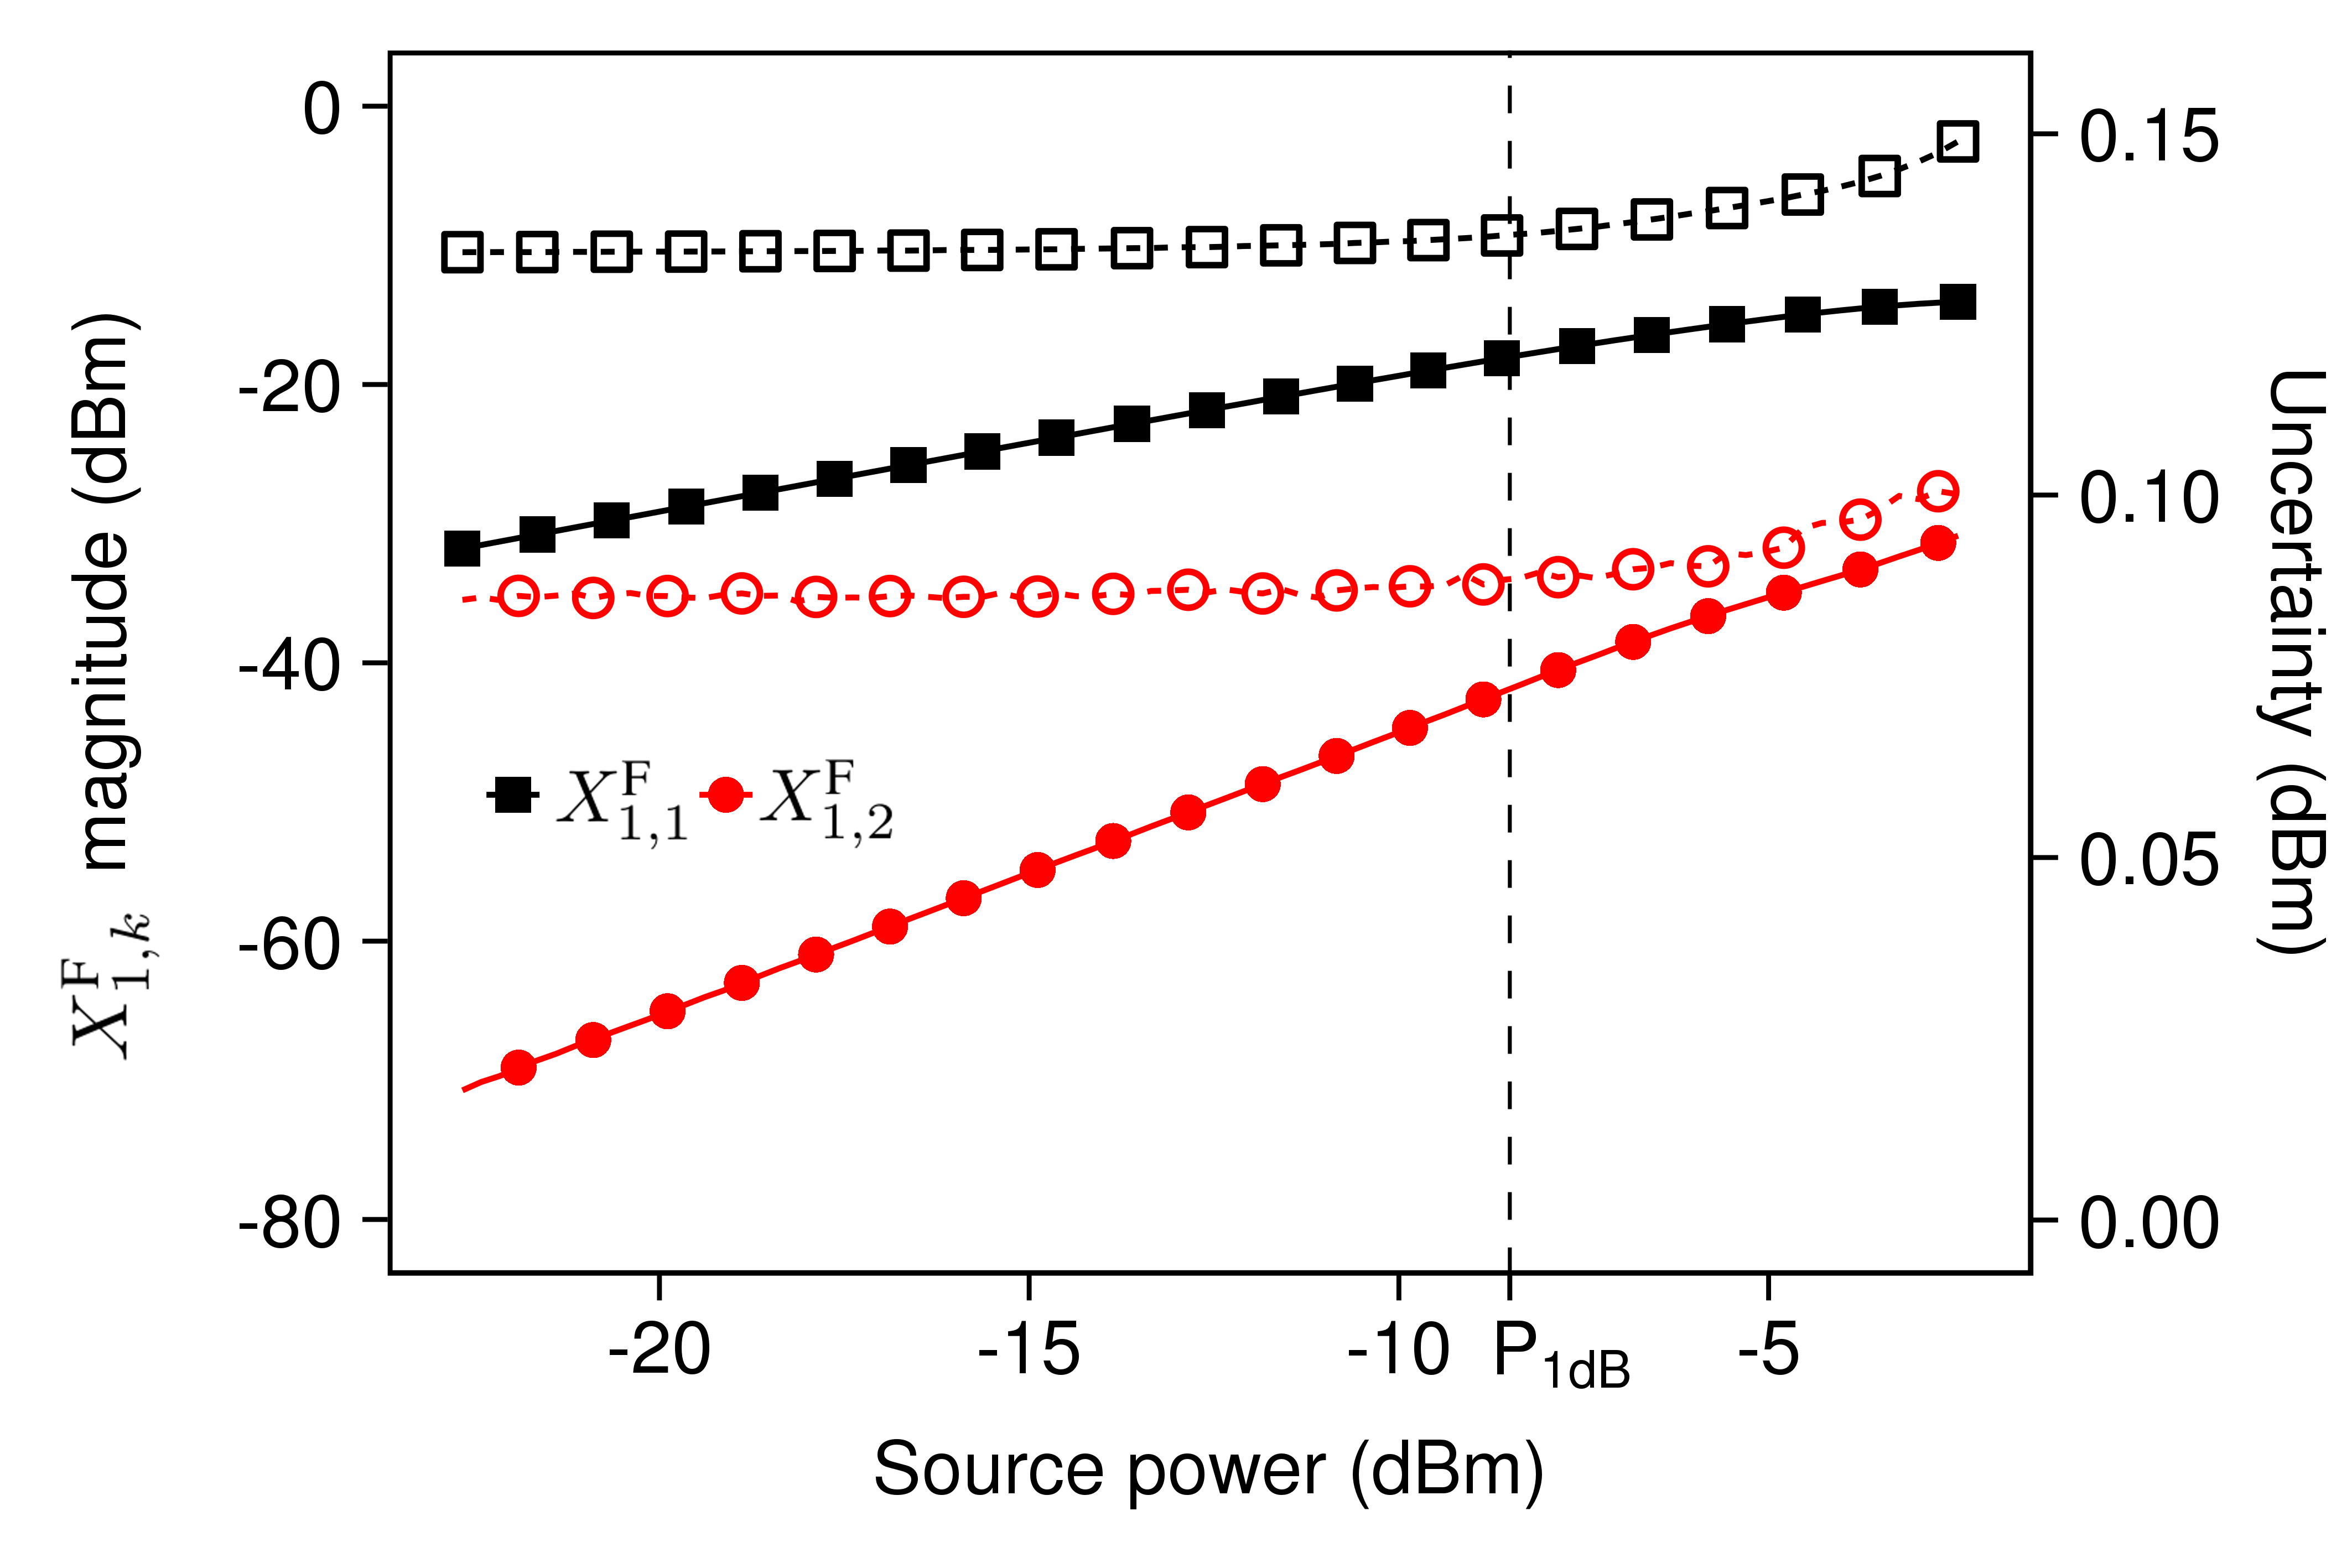
\includegraphics[width=\linewidth,height=5cm]{fig4a}			
		\label{ch5_fig_FB1kdB}
	\end{subfigure}\hfil%
	\begin{subfigure}{0.45\textwidth}
		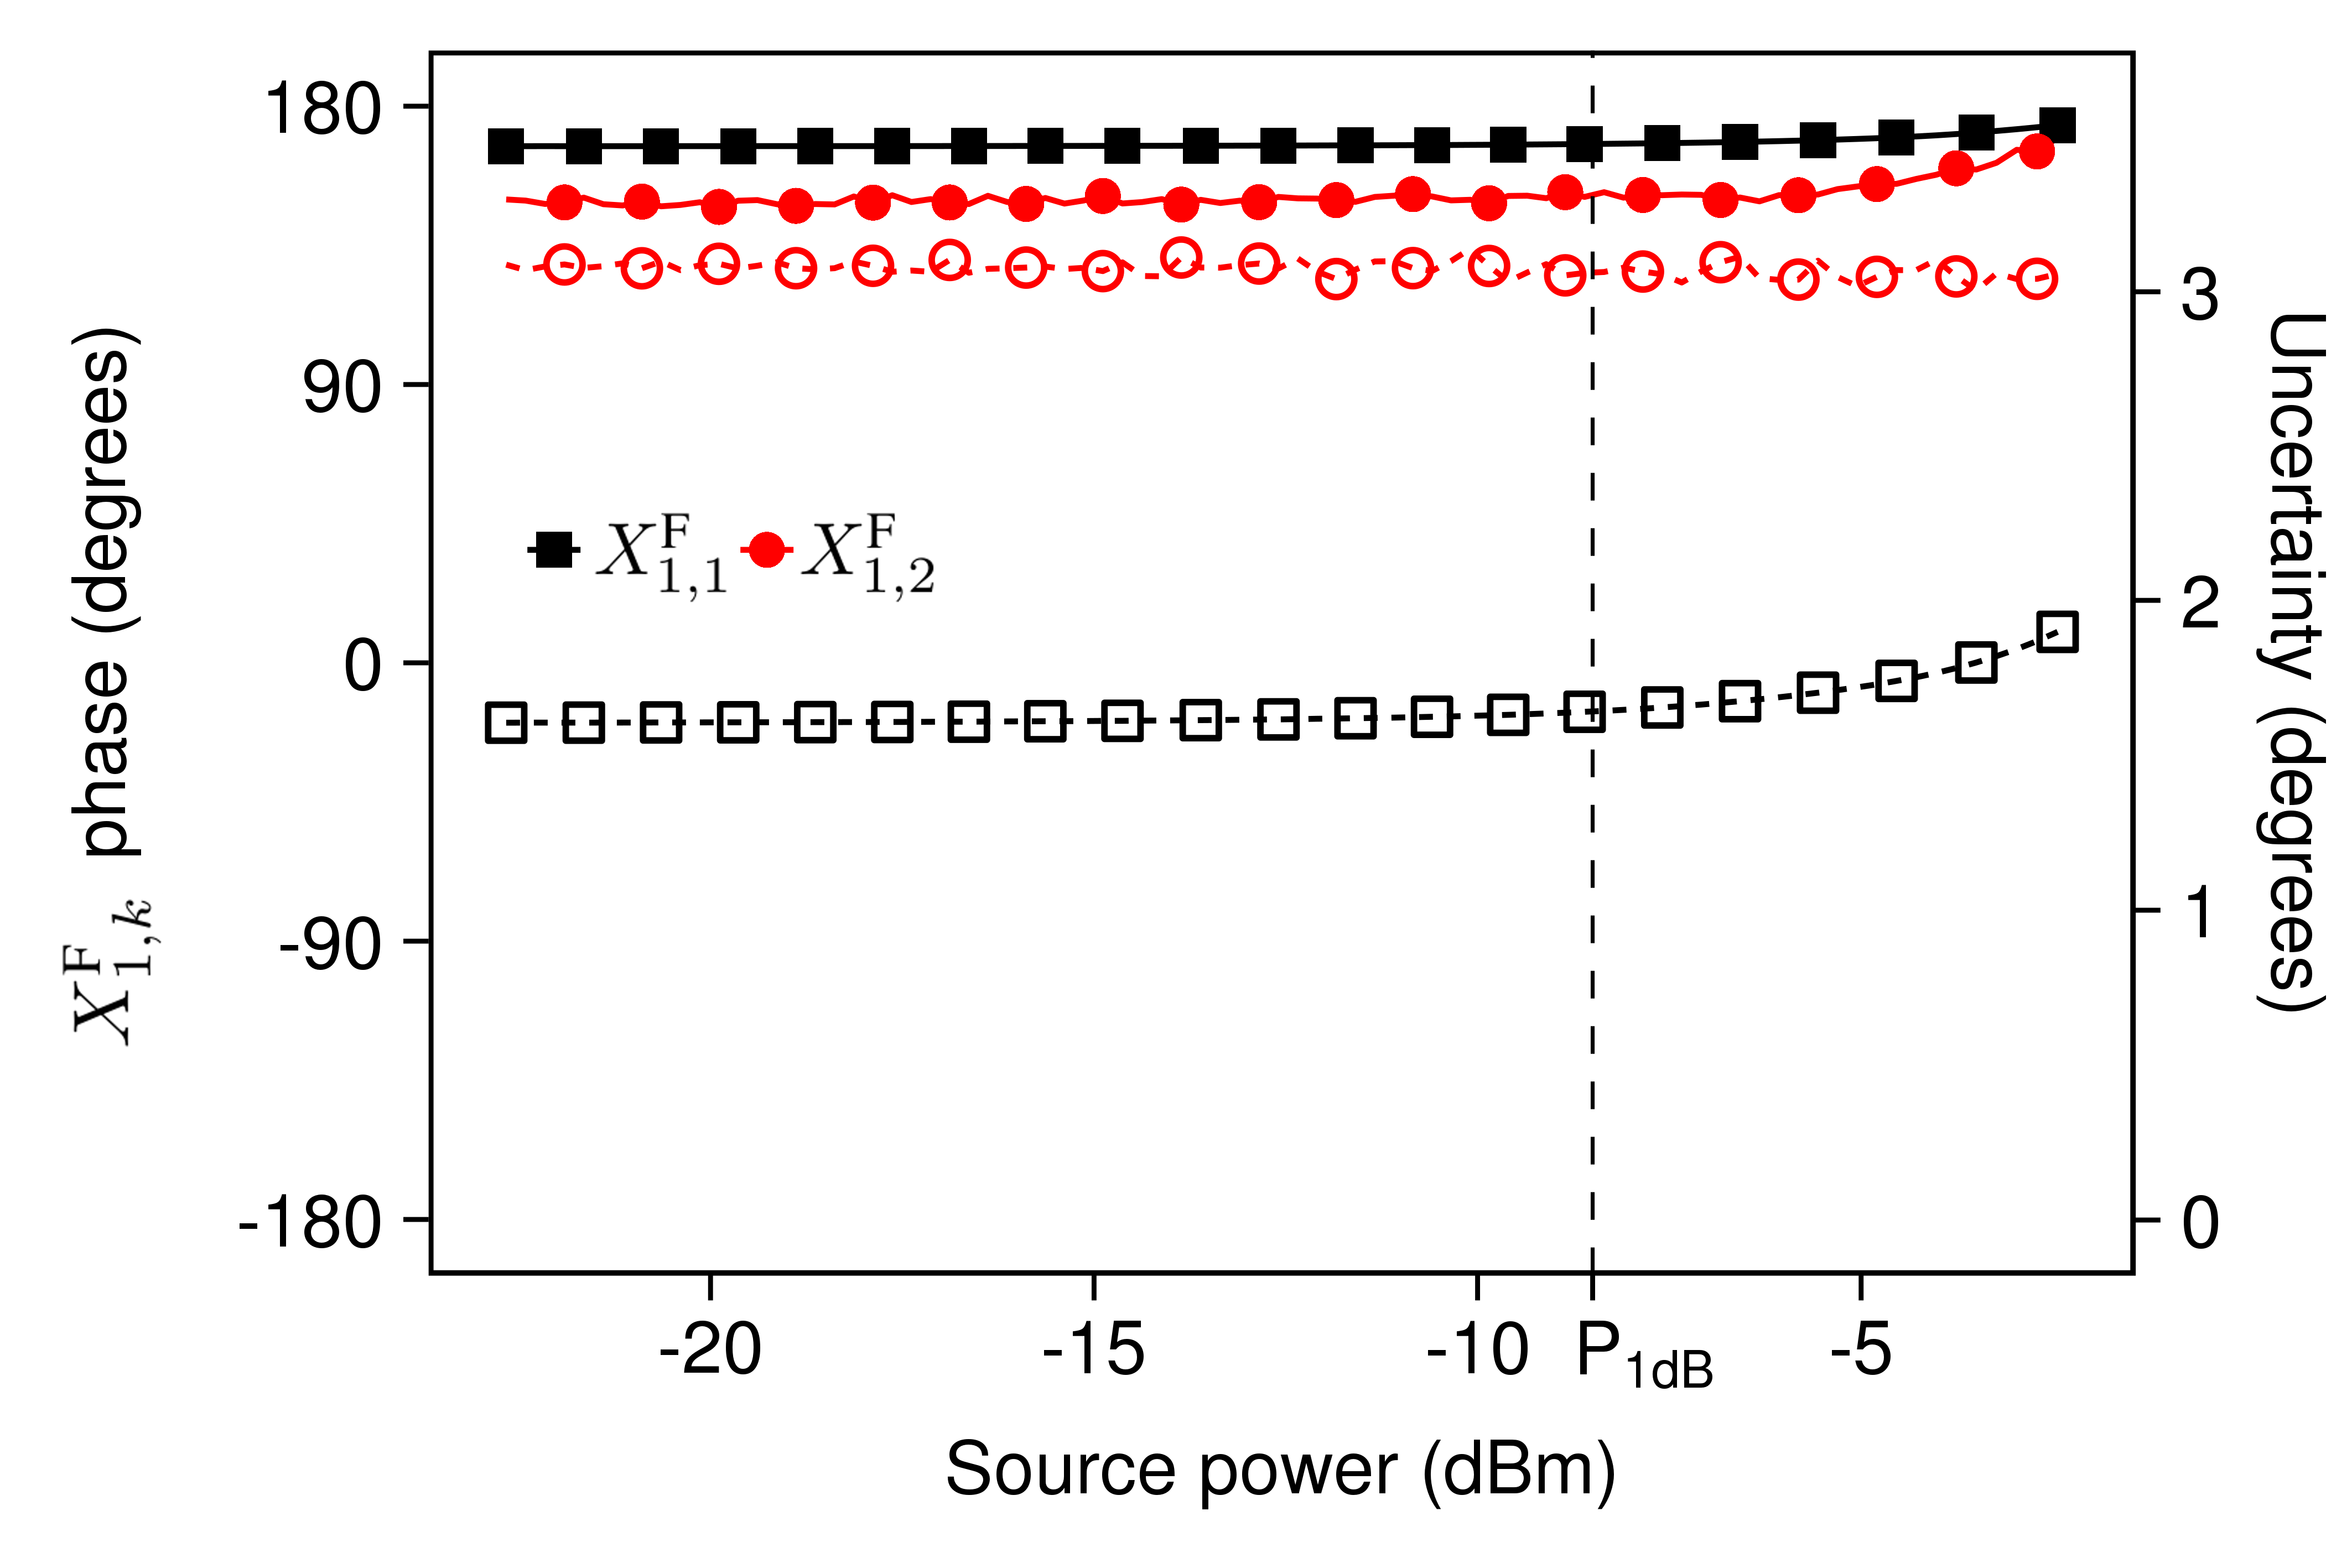
\includegraphics[width=\linewidth,height=5cm]{fig4b}
		\label{ch5_fig_FB1kp}
	\end{subfigure}
	\begin{subfigure}{0.45\textwidth}
		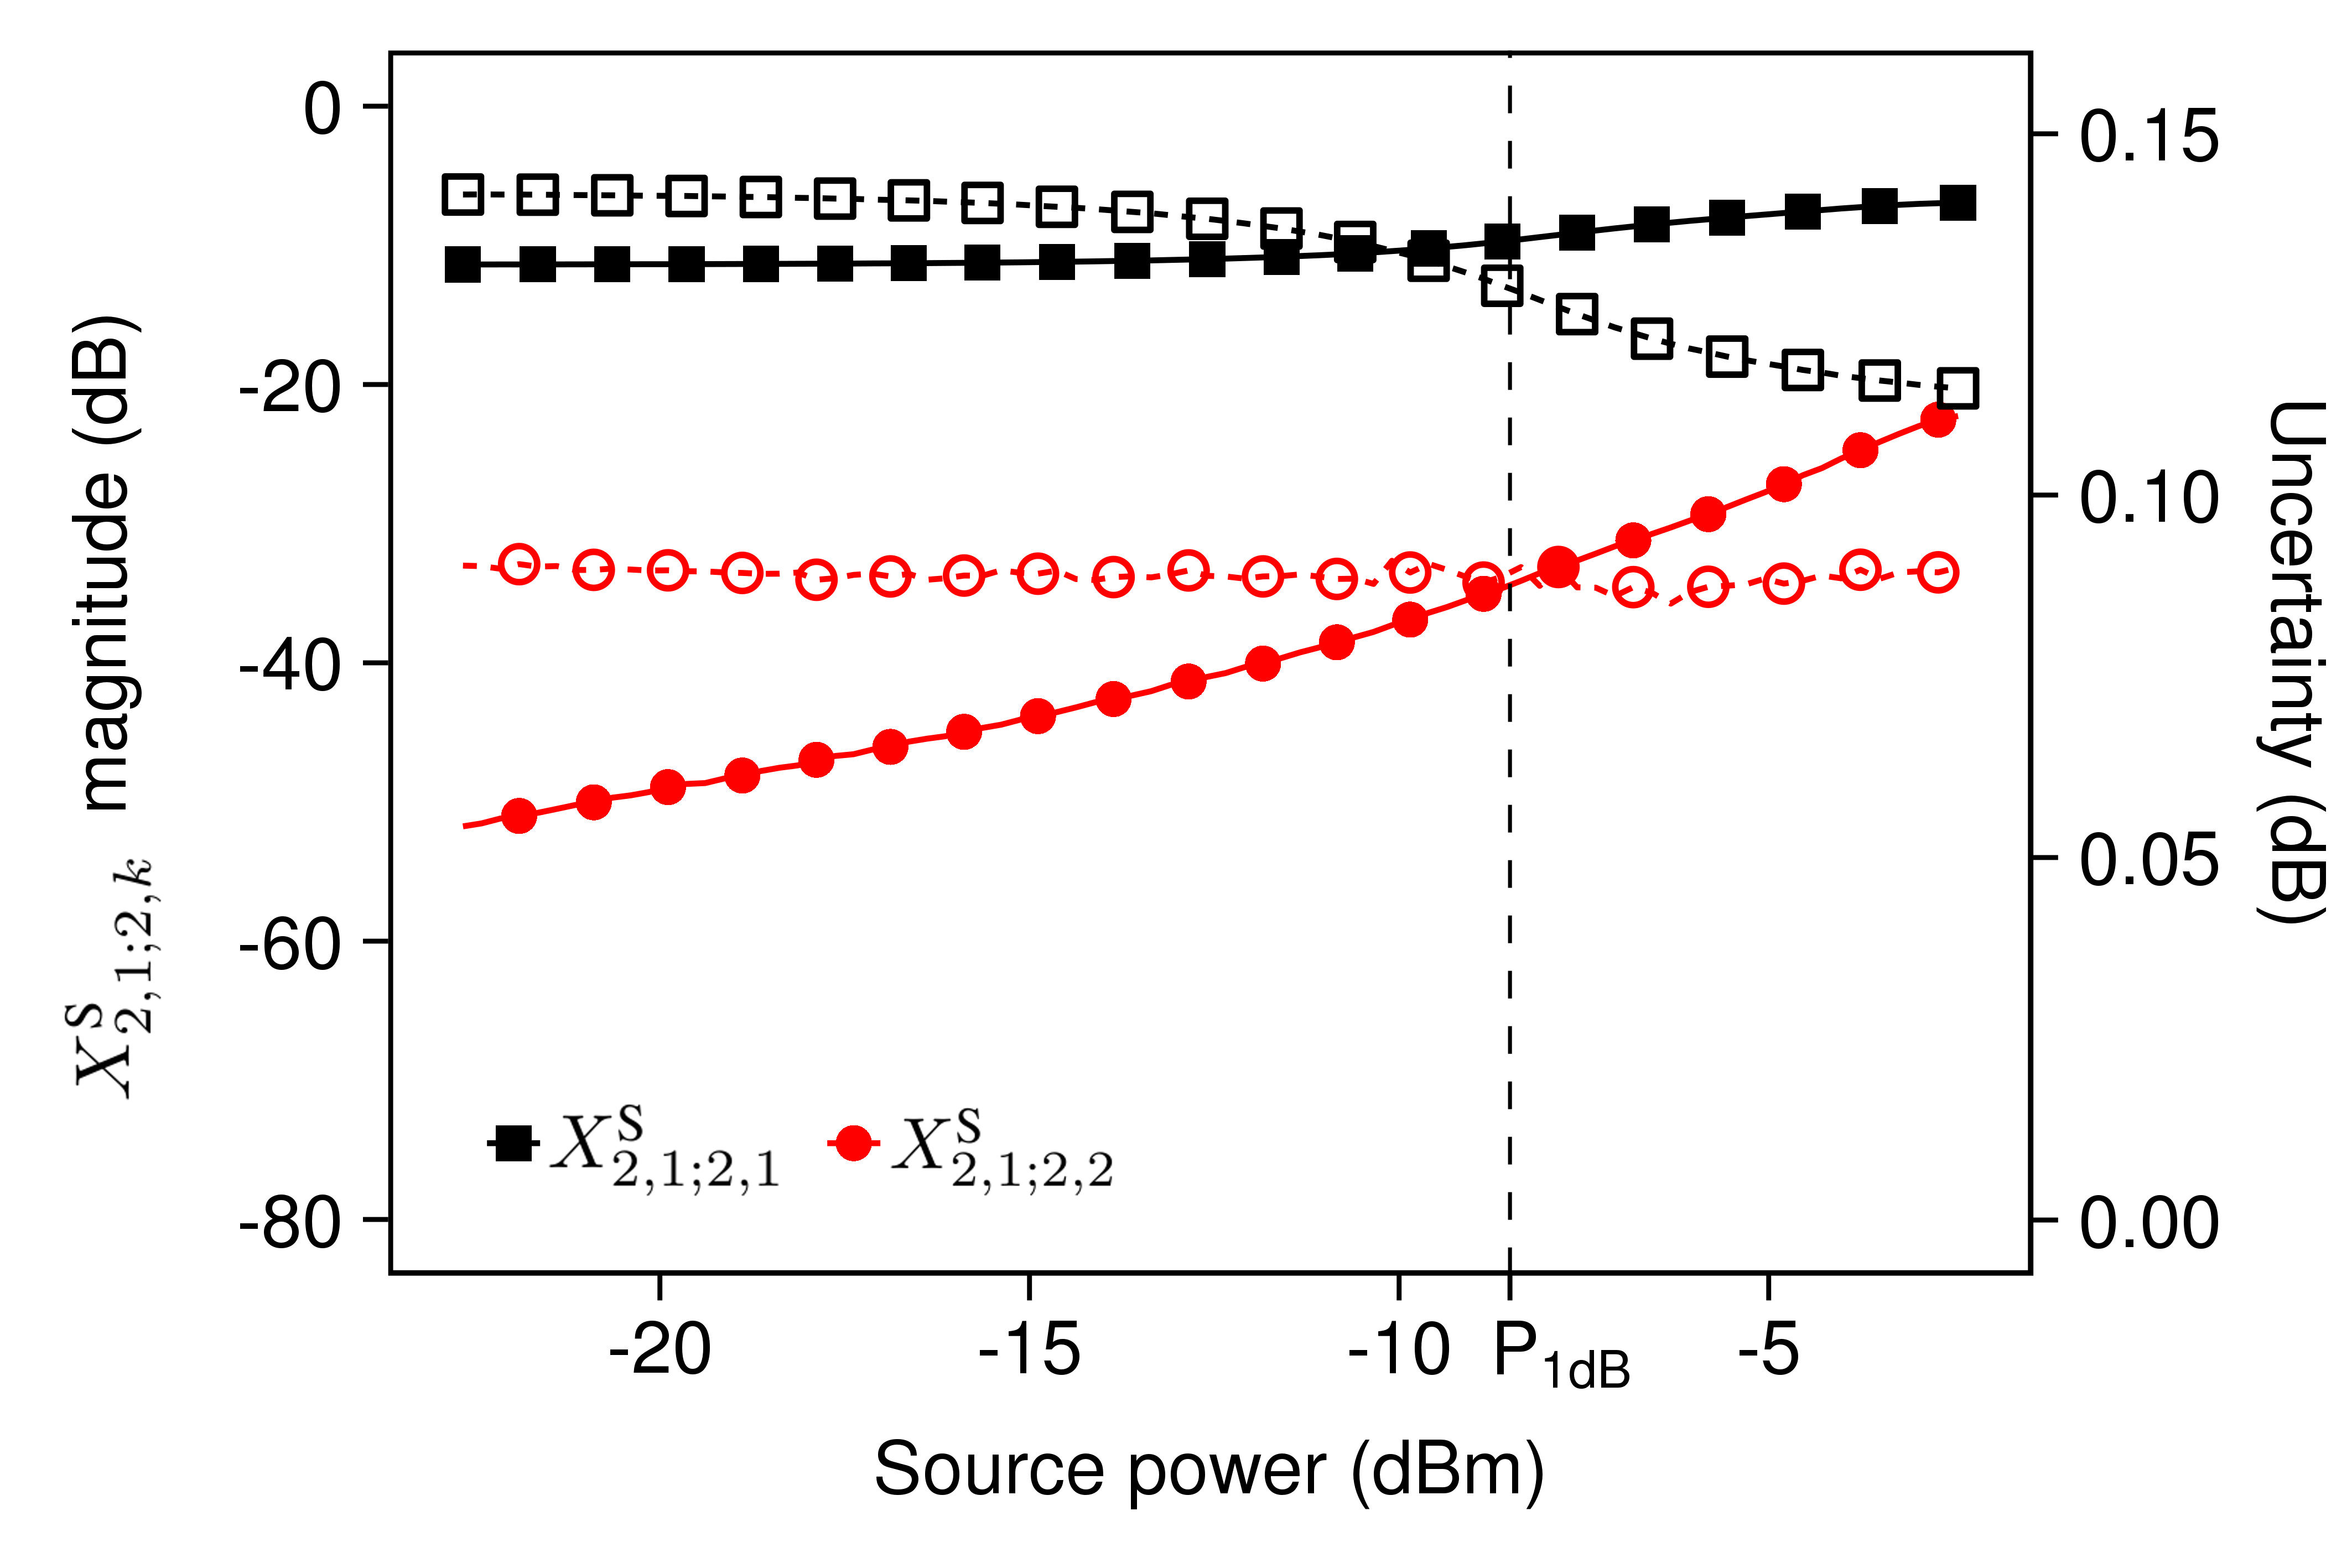
\includegraphics[width=\linewidth,height=5cm]{fig4c}
		\label{ch5_fig_s212kdB}
	\end{subfigure}\hfil%
	\begin{subfigure}{0.45\textwidth}
		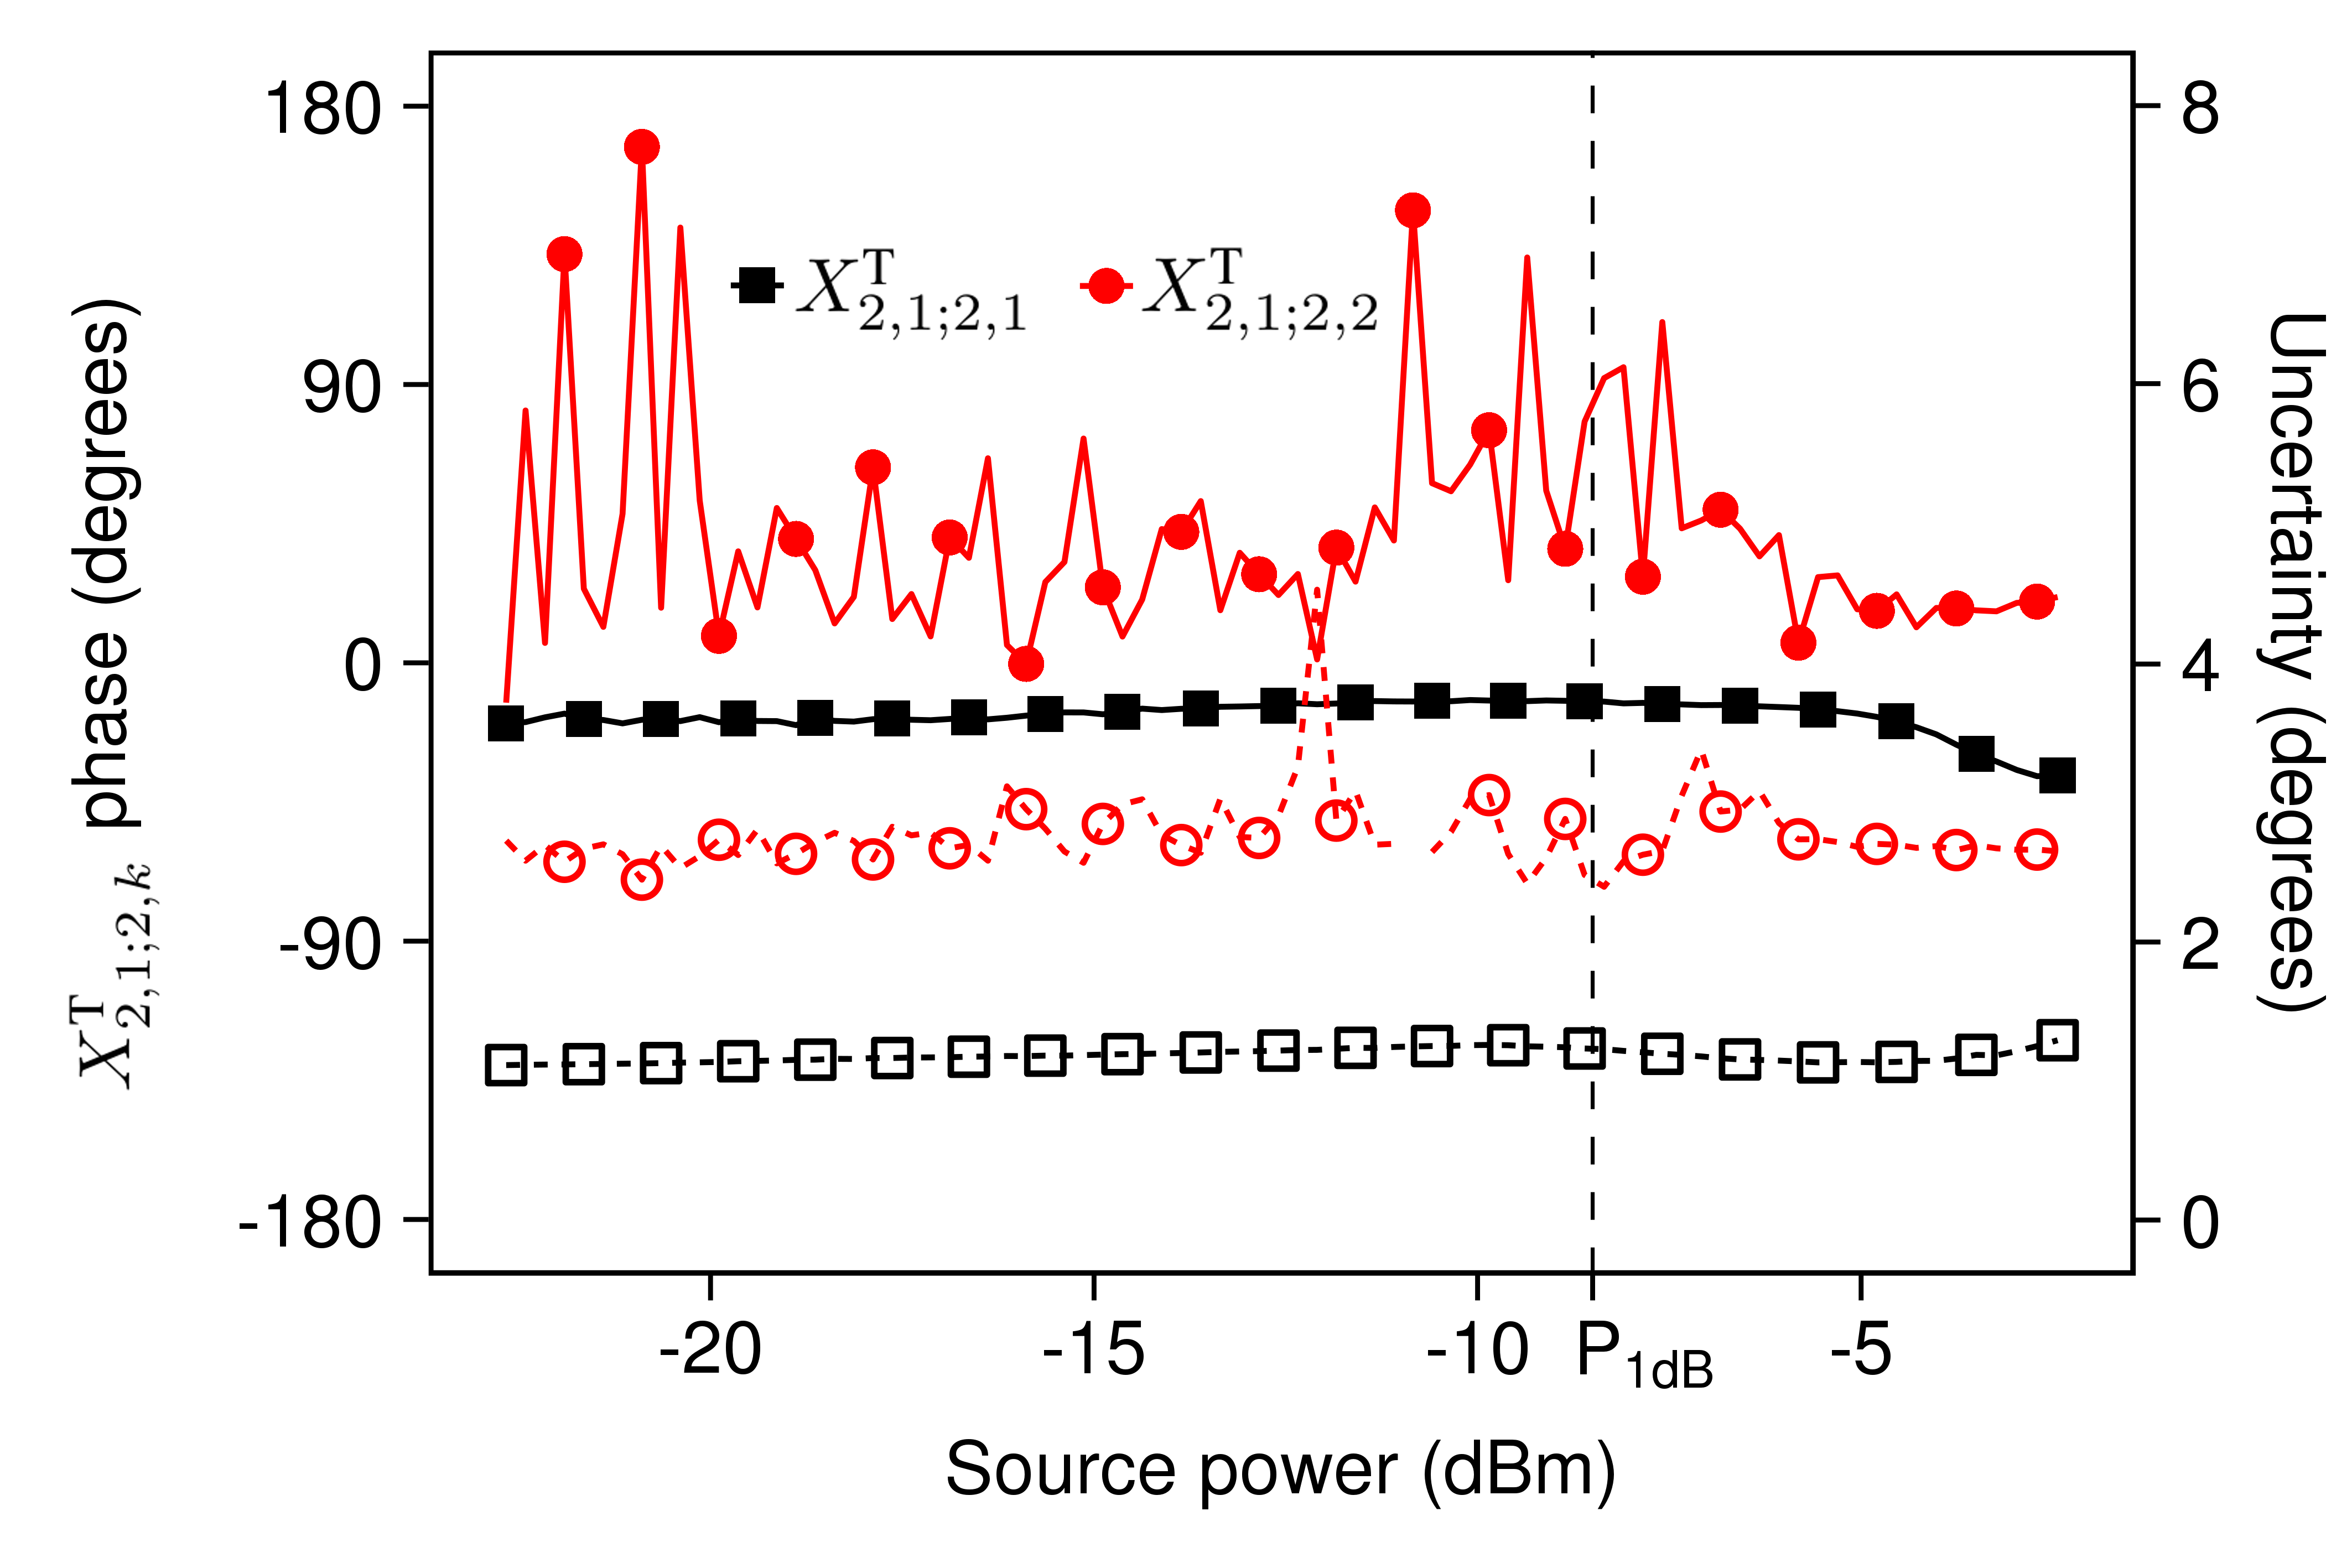
\includegraphics[width=\linewidth,height=5cm]{fig4d}	
		\label{ch5_fig_t212kp}
	\end{subfigure}
	\caption{Estimates (solid line and shapes, left scale) and standard uncertainties (dashed line and hollow shapes, right scale) for the magnitude and phase of a sample of the extracted X-parameters. Harmonic indices 1 and 2 relate to measurement frequencies of 25 and 50 GHz, respectively. Uncertainties are a linear variation of the scale value.}
	\label{ch5_fig_summaryplots}
\end{figure}

\section{Conclusions}

\addcontentsline{toc}{section}{Bibliography}
\printbibliography[title=References]
\end{refsection}
\end{document}
